\cotefile{74}
\scanpage{56}
Sa structure combinatoire est donnée par les ens $I_{\gamma}$ de cardinal 3 et $\deleted{\unsure{\Sigma|I}}\Lambda_{\gamma}=\Lambda-\{\gamma\}\inserted{=\{\alpha,\beta\}}$ de cardinal 2, comme $H\simeq I_{\gamma}\times\Lambda_{\gamma}$, avec $\tau_{\deleted{\unsure{\alpha}}i,\alpha}$ et $\tau_{j\beta}$ \uline{liés} ssi $i\ne j,\ \alpha\ne\beta$. \deleted{\unsure{(deux îlots}}

\diagram{\begin{tikzcd}[ampersand replacement=\&,column sep=small,row sep=small]
\&\tau_{i\alpha}\arrow[r,dash]\&\tau_{j\beta}\arrow[dr,dash]\&\\
\tau_{k\beta}\arrow[ur,dash]\arrow[dr,dash]\&\&\&\tau_{k\alpha}\arrow[dl,dash]\\
\&\tau_{j\alpha}\arrow[r,dash]\&\tau_{i\beta}\&
\end{tikzcd}}

\textcircled{14} Les triangles de triades biliées correspondent aux couples $(\alpha,\beta)$ d'élt. distincts de $\Lambda$ (i.e. aux repères de $\Lambda$) en associant à tt tel repère le \deleted{\unsure{ens de}} triangle de triades $T_{\alpha,\beta,\gamma}\deleted{\unsure{\{\tau_{i,\alpha},\overline{\tau}_{j}}}\ \{\tau_{i\alpha}\}_{i\in I_{\gamma}}$. Cet ens est donc un torseur à droite sous le groupe $\unsure{\mathfrak S_3|\mathscr S_3}$. Ceci dit, \deleted{\unsure{le triangle de}} \inserted{le triangle des} triades \uline{opposé} à $T_{\alpha\beta\gamma}$ est
\[
\overline{T_{\alpha\beta\gamma}}=T_{\beta,\alpha,\gamma}
\]

Le triangle de triades $\widetilde T_{\alpha\beta\gamma}$ \deleted{\unsure{co}} contenu dans le $\unsure{=|\simeq}$ bitriangle $X_\alpha$ que $\deleted{\unsure{X_{\alpha\beta}}}T_{\alpha\beta\gamma}$, et distinct de $T_{\alpha\beta}$, est $T_{\alpha\gamma\beta}$. Donc le groupe engendré par les opérations $-$ et $\sim$ sur l'ens des triangles de triades liées

% archive sheet number: 55

\scanpage{57}
d'un graphe cubique $\Delta$ est isomorphe au groupe $\unsure{\mathfrak S_3|\mathscr S_3}$, avec $-$ correspondant à $\sigma_{12}$, $\sim$ à $\sigma_{23}$ ....

\uline{NB} En \unsure{termes|terme} d'un couple $(X,\{\unsure{\tau_i|\tau_i'}\}_{i\in I})$ d'un bitriangle $X\subset\Delta$ et d'une coorientation de celui-ci, \unsure{les règles|donc presque} précédentes associent à un tel couple, d'une part le
\deleted{couple $(X',(\tau_i')_{i\in I})$ \inserted{\unsure{même} $I$} formé du bitriangle $X'$ associé à $X$, tel que les $\tau_i'$ sont les orbites}
$X'=\bigcup_{i\in I}\overline{\tau_i'}$ \inserted{triade opposée} muni des $(\overline{\tau_i'})_{i\in I}$, d'autre part $X$ muni de l'autre coorientation $(\tau_i')_{i\in I'}$ .....

\deleted{\textcircled{15} \unsure{Pour les triades}}

\textcircled{15} Les triangles de $X_\alpha$ correspondent aux parties $\deleted{\unsure{h}} \inserted{t}\subset\prod_{\beta\in\Lambda-\{\alpha\}} I_\beta$ \deleted{qui sont des} telles que les applications $t\longrightarrow I_\beta$ $(\beta\in\unsure{\Delta|\Lambda}-\{\alpha\})$ \inserted{i.e. (si $\Lambda=\{\alpha,\beta,\gamma\}$) aux bijections $I_\beta\overset{\sim}{\longrightarrow}I_\gamma$} sont bijectives, en associant à une telle \deleted{partie} \deleted{\unsure{l'ens des él.}} \inserted{bijection $\varphi\colon\deleted{\unsure{I}}$} l'ens des él. $\{\{x_\beta,\varphi(x_\beta)\}\}_{x_\beta\in I_\beta}$ de $X_\alpha$. Ceci posé, pour un tel triangle $\underline{t}=\underline{t}_\varphi$, la symétrie correspondante de $\Delta$ est

% archive sheet number: 56

\scanpage{58}
celle associée à l'autom suivant de $(I\xrightarrow{p}\Lambda)$ : son action sur $\Lambda$ est la permutation qui fixe $\alpha$ i.e. échange $\beta,\gamma$, son action sur $I$ est l'identité sur $I_\alpha$, et elle échange en\unsure{tre} eux $x_\beta\in I_\beta$ et $\varphi(x_\beta)$. On voit immédiatement que le groupe engendré par ces opérations est le groupe de tous les autom de $\Delta$ laissant invariant sa partition $\Delta=\bigcup X_\alpha$.

\deleted{Le groupe engendré} Le sous-groupe engendré par les $\sigma_{\underline t}$ avec $t$ \unsure{triang.|triangle} de $X_\alpha$ ($\alpha$ fixé) est formé des autom de $\Delta$ qui a) \unsure{invarient} $X_\alpha$ (donc la partition)
b) opèrent trivialement sur l'ens $\unsure{\tau|=|\pi}(X_\alpha)\simeq I_\alpha$ des ``trois orbites'' associé à $X_\alpha$.

\textcircled{16} Soit $X\subset S$ un bitriangle de $S$, et $\deleted{\unsure{/}}(S_i)_{i\in I_X}$ l'une des ``trois orbites'' de $S-X$.

Alors les sous-graphes \inserted{de type} $\unsure{\mathscr T|\Gamma|\mathcal T}_1$ \deleted{\unsure{$\subset$}} contenant $X$ sont les $X\cup S_i$. Donc la \deleted{\unsure{donnée}} \inserted{\unsure{catég\textsuperscript{rie}|catégorie}} \deleted{\unsure{de leurs}} \unsure{des} triplets $(S\supset\unsure{\mathscr X|\mathfrak X|\mathcal X}\supset X)$ d'un \deleted{\unsure{cubique}} \inserted{graphe}

% archive sheet number: 57

\scanpage{59}
cubique \inserted{$(\unsure{\mathscr T|\Gamma|\mathcal T}_2)$} muni d'un $\mathscr T_1$ et d'un $\mathscr T_0$ contenu dans celui-ci, équivaut à la \deleted{donnée \unsure{d'un}} \inserted{catégorie} \deleted{de} $(\mathrm{Ens})_{3,3}\times(\mathrm{Ens})_2$ \deleted{ens à trois éléments,} \deleted{en associant à un} \inserted{[en associant l'ens des} triades de $X$, et l'ens des deux orbites dans $S-\unsure{\mathscr X|\mathfrak X|\mathcal X}$]

\deleted{couple de} La \deleted{donnée} \inserted{catégorie} des systèmes $(S\supset\mathscr X\supset X\supset t)$ d'un $\mathscr T_2$ contenant un $\mathscr T_1$ contenant un $\mathscr T_0$ contenant un $\mathscr T_{-1}$, équivaut à la catégorie $(\mathrm{Ens})_3\times(\mathrm{Ens})_2\times(\mathrm{Ens})_2$, [en lui associant l'ens des points de l'une des triades de $\deleted{\unsure{X|\mathscr X|\mathcal X}}$ pour la relation d'équiv. définie par $t$, l'ens des deux coorientations de $X$, et l'ens des deux orbites de $S-\mathscr X$] ....

\textcircled{17} Soit $\mathscr X$ un $\mathscr T_1$ dans \deleted{\unsure{$S$}}\unsure{un|le} $\mathscr T_2$ $S$. Alors $S-\mathscr X$ est une bibase de $S$, et on trouve ainsi une bijection entre l'ens des $\mathscr T_1$ de $S$, et l'ens des bibases.
La catégorie des $\mathscr T_2$ munis d'une bibase, celle des $\mathscr T_2$ munis d'un $\unsure{\mathscr X_1|\mathcal X_1}$, et la catégorie des $(\mathrm{Ens})_6\times(\mathrm{Ens})_2$, sont canoniquement équivalentes.

% archive sheet number: 58

\scanpage{60}
\textcircled{18} À tout $B\in(\mathrm{Ens})_6$, ensemble de cardinal 6, associons le graphe $\unsure{\mathscr T|\Gamma|\mathcal T}_1(B)$ suivant
\[
\left\{\begin{aligned}
&\text{ens sommets}=\unsure{\mathfrak P|\mathscr P}_2(B)\\
&\deleted{A,B,}\ u,v\in\mathfrak P_2(B)\quad\text{liés ssi}\quad u\cap v=\varnothing
\end{aligned}\right.
\]

Alors $\mathscr T_1(B)$ est un graphe \unsure{trilétaire|trialitaire|trilitaire|tritétraèdre} donc un $\mathscr T_1$, et le foncteur $B\longrightarrow\mathscr T_1(B)$ est une équivalence de la catégorie $(\mathrm{Ens})_6$ avec la catégorie des $\mathscr T_1$. Le foncteur quasi-inverse associe à $\unsure{\mathscr X|\mathfrak X|\mathcal X}$ l'ens $\underline{B}$ des parties discrètes de card 5 de $\mathscr X$.
Alors tt $x\in\mathscr X$ est contenu dans exactement deux éléments de $B$, et l'application $\mathscr X\mathbin{\unsure{-|\longrightarrow}}\mathfrak P_2(B)$ ainsi obtenue est un isom. du graphe $\mathscr X$ avec le graphe $\mathscr T_1(B)$.
La donnée d'un bitriangle de $\mathscr X$ équivaut à la donnée d'une partition de type $3,3$ de $B$ -- à celle-ci correspond l'ens des \deleted{\unsure{parties}} \inserted{$\in\mathfrak P_2(B)$} qui sont des sections de $B$ sur l'ens \unsure{quot\textsuperscript{t}} à deux éléments.
Tout bitriangle a un $\mathscr T_2$ enveloppe canonique (le foncteur des $(\mathscr X,X)$ d'un $\mathscr T_1$ et d'un $\mathscr T_0$ contenu, vers les $X$, est une équivalence de catégories).

% archive sheet number: 59

\scanpage{61}
19) Considérons \deleted{\unsure{$G$ un}} \inserted{graphe} cubique $\Delta$ avec partition \unsure{trialitaire|trilétaire|tritétraèdre} $S=\bigcup_{\alpha\in\Lambda}X_\alpha$, et considérons le \unsure{gpe|groupe} $G\ (\simeq\unsure{\mathfrak S_3|\mathscr S_3}\mathbin{.}(\mathfrak S_3\times\mathfrak S_3\times\mathfrak S_3))$ des autom de $S$ ainsi décomposé, $\deleted{\unsure{G}}$ et son opération sur l'ens \inserted{$(\mathrm{Tria})$} des triades de $\Delta$, \inserted{et sur l'ens des (\unsure{bitr|bitri}) des bitriangles de $\Delta$.} Alors \deleted{il y a}

a) \deleted{existent} \inserted{Il y a} \deleted{trois} \inserted{quatre} orbites de $G$ sur Tria :

1°) L'orbite formée des triades contenues dans un des $X_\alpha$

2°) L'orbite \deleted{formée} des triades de la forme
\diagram{\begin{tikzcd}[ampersand replacement=\&,row sep=small,column sep=large]
\bullet\arrow[r,dash]\&\bullet\arrow[ddl,dash]\&\bullet\&\\
\bullet\&\bullet\arrow[r,dash]\&\bullet\&\text{(type I)}\\
\bullet\&\bullet\&\bullet\&
\end{tikzcd}}

3°) L'orbite \deleted{formée} des triades de la forme
\diagram{\begin{tikzcd}[ampersand replacement=\&,row sep=small,column sep=large]
\bullet\arrow[r,dash]\arrow[dr,dash]\&\bullet\&\bullet\&\\
\bullet\&\bullet\&\bullet\&\text{(type II)}\\
\bullet\&\bullet\arrow[r,dash]\&\bullet\&
\end{tikzcd}}

4°) L'orbite des triades de la forme
\diagram{\begin{tikzcd}[ampersand replacement=\&,row sep=tiny,column sep=small]
\bullet\arrow[rr,dash,bend left=12]\&\bullet\&\bullet\&\\
\bullet\&\bullet\arrow[r,dash]\&\bullet\&\text{(type III)}\\
\bullet\arrow[r,dash]\&\bullet\&\bullet\&
\end{tikzcd}}

b) Les triades contigues à une triade de type II sont de type I, celles contigues à une triade de type I sont de type I l'une, de type II l'autre de sorte que \deleted{\unsure{un}} l'hexagone \deleted{de triades} \inserted{d'une triade de type I ou II} est de type
\diagram{\begin{tikzcd}[ampersand replacement=\&,row sep=tiny,column sep=small]
\&\mathrm I\arrow[r,dash]\&\mathrm{II}\arrow[dr,dash]\&\\
\mathrm{II}\arrow[ur,dash]\arrow[dr,dash]\&\&\&\mathrm{II}\arrow[dl,dash]\\
\&\mathrm{II}\arrow[r,dash]\&\mathrm I\&
\end{tikzcd}}
(2 sommets \inserted{opposés} de type I, les autres de type II), l'hexagone d'une triade de type (III) est \inserted{formé de triades} de type III

% archive sheet number: 60

\scanpage{62}
Voici un hexagone \deleted{de triades} \inserted{(\deleted{\unsure{typi}}typique) dont une triade (donc \unsure{ttes})} \deleted{\unsure{dont}} \deleted{non} \inserted{n'est \deleted{\unsure{contenue}}} contenue dans aucun des $X_\alpha$ [on note $(i,j,k)$ $(p,q,r)$ $(s,t,u)$ les trois fibres de $I\longrightarrow\Lambda=\{1,2,3\}$]

\diagram{\begin{tikzcd}[ampersand replacement=\&,row sep=small,column sep=small]
\&\substack{\mathrm{II}\\(ip)(uj)(uk)}\arrow[dl,dash]\arrow[dr,dash]\&\\
\mathrm I\quad(i\unsure{r|v})(qs)(qt)\arrow[d,dash]\&\& (iq,rs,rt)\quad\mathrm I\arrow[d,dash]\\
\mathrm I\quad(\deleted{\unsure{qi|q}}\unsure{qu|qi},\unsure{kr|hr|km},jr)\arrow[dr,dash]\&\& (ru)(kq)(jq)\quad\mathrm I\arrow[dl,dash]\\
\&\substack{(pu)(ti)(si)\\\mathrm{II}}\&
\end{tikzcd}}

Tout triangle de triades \inserted{liées} est formé, soit de triades d'un $\unsure{=|\simeq}$ $X_\alpha$ (de réunion $X_\alpha$), soit de triades de type I \uline{et} II \inserted{(\unsure{2|1} de type I, et 1 de type II)}, soit de triades de type III. \deleted{Dans tout} L'intersection du bitriangle correspondant avec deux des $X_\alpha$ est un doublet, avec le troisième c'est une étoile de triangles à deux branches

\diagram{\begin{tikzcd}[ampersand replacement=\&,row sep=tiny,column sep=tiny]
\bullet\arrow[r,dash]\arrow[ddr,dash]\&\bullet\arrow[dd,dash]\&\bullet\arrow[dr,dash]\arrow[ddl,dash]\&\\
\&\&\&\bullet\arrow[dll,dash]\\
\&a\&\&
\end{tikzcd}}
. \deleted{\unsure{Cet ens|Cela \illegible{1}}}

\deleted{Pour une \deleted{\unsure{bitriangle}} \inserted{telle étoile $E$} donnée dans $X$ il y a exactement trois bitriangles de $S$ coupant $X$ suivant $E$. pour un doublet donné dans $X$, il y a exactement $2\times3$}

\diagram{\begin{tikzcd}[ampersand replacement=\&,row sep=tiny,column sep=large]
\&\&s\arrow[dd,dash]\\
i\arrow[dd,dash]\arrow[dr,dash,"{(a)}"]\&\&\\
\&p\arrow[dd,dash]\&t\arrow[dd,dash]\\
j\arrow[dd,dash]\arrow[dr,dash]\arrow[drr,dash]\arrow[dddr,dashed,no head]\&\&\\
\&q\arrow[dd,dash]\arrow[r,dash]\&u\\
k\arrow[ur,dashed,no head]\arrow[urr,dashed,no head]\arrow[dr,dash]\&\&\\
\&r\arrow[uur,dash]\&
\end{tikzcd}}

$\deleted{\unsure{=(3\times\frac{3!}{2})=54|(3\times\frac{3!}{2})=54}}$

% archive sheet number: 61

\scanpage{63}
Les bitriangles sont en corr. biunivoque avec l'ens des \inserted{couples $(a,u)$ d'un} sommet de $\Delta$, \deleted{en associant à un tel sommet la réunion de} \inserted{et d'un \deleted{\unsure{orb}}} élément $u\in\deleted{\unsure{\mathrm{II}|\Pi}}I(X_\alpha)=I_\alpha$ où $X_\alpha\ni a$ et $I(X_\alpha)=I_\alpha$ est l'ens des trois orbites \unsure{associé|associés|associées}.
À un couple $(a,u)$ correspond le bitriangle formé de $a$, des 4 sommets liés à $a$ dans $X_\alpha$, et des 4 sommets de $S$ qui sont dans l'orbite choisie $u$, et qui sont non liés à $a$.
Pour un $a\in X=X_\alpha$ donné, il y a donc exact\textsuperscript{mt} 3 bitriangles $Y$ qui coupent $X$ suivant la réunion des deux triangles de $X$ de sommet $a$ ; et pour un doublet donné $\{a,b\}$ de $X$ ($a\ne b$, $a$ non lié à $b$) il existe exact\textsuperscript{mt} $\deleted{\unsure{2}}3\deleted{\unsure{6}}$ bitriangles $Y$ coupant $X$ en $\{a,b\}$. [Cela donne

\diagram{$\begin{array}{@{}lr@{}}
\text{\deleted{les trois}}&\\
\text{le bitriangle } X&1\\
\text{les 2 bitriangles } X',X''\ \text{disjoints de } X&2\\
\text{les }3\times9\ \text{bitriangles }Y\text{ coupant }X\text{ suivant une}&27\\
\qquad\text{2-étoile de triangles}&\\
\text{les }\unsure{3|6}\times\deleted{\unsure{10|9}}\unsure{18|9}\ \text{bitriangles }Y\text{ coupant }X\text{ suivant}&54\\
\qquad\text{un doublet}&\deleted{\unsure{90|84}}\\
\text{les }\deleted{\unsure{9\times4}}\inserted{6\times6}\ \text{bitriangles }Y\text{ coupant }X&\\
\qquad\text{suivant un triangle}&36\\ \cline{2-2}
\text{\deleted{\uline{NB} il y a}}&120
\end{array}$}

On avait \deleted{\unsure{oublié}} négligé de détailler le cas des $Y$ engendrés par des triades de type III, plus simple.

% archive sheet number: 62

\scanpage{64}
On trouve qu'ils correspondent au cas de \deleted{\unsure{un syst.}} la figure ci-contre, correspondant à un syst. transitif d'isom entre les $I_\alpha$ (définis par les triangles intersection $Y\cap X_\alpha$).

\diagram{\begin{tikzcd}[ampersand replacement=\&,column sep=tiny,row sep=tiny]
\&\& {}\arrow[dd,dash]\arrow[dl,dash]\\
{}\arrow[urr,dash]\arrow[r,dash]\arrow[dd,dash]\&{}\arrow[dd,dash]\&\\
\&\&{}\arrow[dd,dash]\arrow[dl,dash]\\
{}\arrow[urr,dash]\arrow[r,dash]\arrow[dd,dash]\&{}\arrow[dd,dash]\&\\
\&\&{}\arrow[dl,dash]\\
{}\arrow[urr,dash]\arrow[r,dash]\&{}\&
\end{tikzcd}}

Pour tt triangle donné de $X_\alpha$ (correspondant à une bijection $I_\beta\mathbin{\unsure{-|\longrightarrow}}I_\gamma$) il y en a 6.

\begin{center}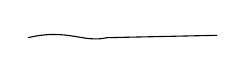
\begin{tikzpicture}\draw (0,0) .. controls (.5,.12) and (.7,-.07) .. (1,0) -- (2.4,.03);\end{tikzpicture}\end{center}

Étudier plus génér\textsuperscript{t}.

a) Position relative de 2 $\unsure{\mathscr T|\Gamma|\mathcal T}_i$ $(-1\le i\le1)$ dans un $\mathscr T_2$

b) Position relative d'une base et d'un $\mathscr T_i$.

\textcircled{20} (\unsure{Variante}) Soit $\tau=\{a,b,c\}$ une triade du $\mathscr T_2$ $\Delta=(S,A)$. Alors \deleted{\unsure{$B$ l'ens}} il y a exactement un bitriangle contenant $t$, qui est aussi formé des él. de $\tau$ et de \inserted{l'ens} des 6 él. de $S-\tau$ qui sont liés à \deleted{au moins} \inserted{exactement} \deleted{\unsure{un}} \inserted{deux} él. de $\tau$ \deleted{(ils sont liés \unsure{en|aux} \inserted{alors}, en fait, à deux tels éléments)}.
Alors $X-\tau=Y$ est un \deleted{hexagone} \unsure{bitripode|bitriade|distingué} i.e. un hexagone. On trouve ainsi une bijection de l'ens des triades sur l'ens des hexagones.

% archive sheet number: 63

\scanpage{65}
La bijection inverse est celle qui associe à tt hexagone $Y$ l'ens $\tau$ des $s\in S-Y$ qui sont liés à au moins un élément de $Y$ (ils sont liés alors à exact\textsuperscript{mt} 4 éléments \inserted{opposés deux à deux} de l'hexagone, 2 sur chacun de ses triangles inscrits, et ils correspondent biunivoqu\textsuperscript{mt} aux trois diagonales de l'hexagone).

Autre procédé (qui revient au précédent, en remplaçant la triade $\tau$ par son opposée $\overline\tau$) : On prend l'ens des $s\in S-\overline\tau$ qui sont non-liés à tous les \unsure{éls|él|él.} de $\overline\tau$, \deleted{\unsure{et}} c'est \deleted{un} \inserted{le} $\unsure{=|\simeq}$ hexagone, \deleted{\unsure{est en somme associé}} que précéd\textsuperscript{mt} (rappelons que $\overline\tau$ est l'ens des él. de $S$ liés à tous les él. de $\tau$).

\uline{Ou encore} Pour une triade donnée $\unsure{\tau|I}$, et $x\in S-\tau$, regardons \deleted{\unsure{le nb}} $\operatorname{Card}\underbrace{\operatorname{Ét}(x)\cap\tau}_{\text{ens des }s\in\tau\text{ liés à }x}$ \unsure{,|]} soit $\unsure{\nu|v}_\tau(x)$.

\uline{Il y a} 6 él. tels que $\nu_\tau(x)=0$, ils forment un hexagone $h(\tau)$

9 él. tels que $\nu_\tau(x)=1$, ils forment un bitriangle $\mathrm{bit}(\tau)$

6 él. tels que $\nu_\tau(x)=2$, ils forment un hexagone $\overline h$ (dit ``opposé'' à $h$) $\overline h(\tau)$

3 él. tels que $\nu_\tau(x)=3$, ils forment une triade $\overline\tau$ (dite ``opposée'' à $\tau$).

% archive sheet number: 64

\scanpage{66}
On \unsure{a|.}
\[
\mathrm{bit}(\tau)=\mathrm{bit}(\overline\tau)=\mathrm{bit}(\unsure{\tau'_6|\tau'})=\mathrm{bit}(\tau'')=\mathrm{bit}(\overline\tau')=\mathrm{bit}(\overline\tau'')
\]

% slanted
\margin{détailler tout ça dans énoncés en forme ....}
où $\tau',\tau''$ sont les triades composantes de l'hexagone $h(\tau)$, de sorte que $\overline\tau',\overline\tau''$ sont les triades composantes de l'hexagone $h(\overline\tau)=\overline h(\tau)$.

% archive sheet number: 65

\scanpage{67}
\diagram{\begin{tikzcd}[ampersand replacement=\&,column sep=small,row sep=small]
\&\unsure{t''|t'|b'}=A_4\arrow[dl,dash,very thick]\arrow[rr,dash]\arrow[dr,dash]\&\&t=A_3\arrow[dl,dash]\arrow[dr,dash]\&\\
2:\unsure{u'|v'|a'}\arrow[dr,dash]\&\&b\arrow[dl,dash]\arrow[dr,dash]\&\&\unsure{s|g}=A_2\arrow[dl,dash,thick]\\
\&c=A_0\arrow[rr,dash,very thick]\&\&a=A_1\&
\end{tikzcd}}

\diagram{\begin{tikzcd}[ampersand replacement=\&,row sep=tiny,column sep=tiny]
{\unsure{\zeta|\gamma|\xi}}_1\arrow[dr,dash]\arrow[drr,dash]\&\zeta_2\arrow[dl,dash]\arrow[dr,dash]\&\zeta_3\arrow[dll,dash]\arrow[dl,dash]\\
\zeta'_1\&\zeta'_2\&\zeta'_3
\end{tikzcd}}

\diagram{\begin{tikzcd}[ampersand replacement=\&,column sep=normal,row sep=small]
\zeta_1\arrow[dr,dash]\arrow[drr,dash]\&\zeta_2\arrow[dl,dash]\arrow[dr,dash]\&\zeta_3\arrow[dll,dash]\arrow[dl,dash]\\
\zeta'_1\&\underset{\rule{.4pt}{.65ex}\rule{1.1em}{.4pt}\rule{.4pt}{.65ex}}{\zeta'_2}\&\zeta'_3
\end{tikzcd}}

$\unsure{z'|\tau'}\in\widetilde E_{c}$ lié à $\unsure{g|s}$ et à $t$

\[
\overset{\tikz{\draw (0,-.12)--(0,0)--(2.2,0)--(2.2,-.12);}}{27\mathbin{.}10\mathbin{.}8}\mathbin{.}4\mathbin{.}1\mathbin{.}2
\]

\[
\begin{aligned}
2^7\mathbin{.}3^3\mathbin{.}5&=\text{Nb de hexagones épinglés}\\
2^6\mathbin{.}3\mathbin{.}5&=\text{Nb des hexagones}=\text{Nb des bitriades}
\end{aligned}
\]

$\unsure{\nearrow|\rightleftarrows}$ elles sont conjuguées \unsure{é}

La donnée d'un $A_4$ ($\Longleftrightarrow$ d'un $A_5$) est équivalente à celle d'un \uline{bitriangle épinglé} dans $S$

$\deleted{(a,b,c)}$ $\deleted{(x,y,z)}$ $\deleted{\unsure{u,v,}}$

\[
 A_4\Longleftrightarrow A_5\Longleftrightarrow P_6\Longleftrightarrow \text{bitriade épinglée}
\]

\deleted{Nb de bitriades épinglées} \inserted{bitriades sont conjugués}

\deleted{\unsure{tout}} \deleted{Nb de bitriades} \deleted{Nb de}
\[
\text{Card bitriad}=\left(\frac{12}{72}\right)\inserted{\frac16}\text{Nb des bitriangles}
\]

\[
\deleted{\unsure{\mathrm{Les}}}\quad\deleted{27\mathbin{.}16\mathbin{.}8=3\mathbin{.}720}
\inserted{27\mathbin{.}16\mathbin{.}10=6\mathbin{.}720}=\text{Nb des triades épinglées}
\]

\unsure{Nb|NB}

\[
\begin{aligned}
45\times16=720&=\text{Nb des bitriangles munis d'un triangle}\\
&\deleted{=\text{Nb de triades}}\\
&=\text{Nb de triades}
\end{aligned}
\]

\[
\text{Nb de bitriangles}=120
\]

% archive sheet number: 66

\scanpage{68}
% letterhead
Séminaire Nicolas BOURBAKI

19, 20, 21 juin 1976 - Amphi. Hermite - 14 H 30

Institut Henri Poincaré - 11 rue P. et M. Curie

\uline{PARIS 5e}

\uline{Samedi 19 juin}

A. GRAMAIN - Rapport sur la théorie des noeuds.

A. GUICHARDET - Représentations des groupes $\mathrm G^{\mathrm X}$ d'après Gelfand et Delorme.

\uline{Dimanche 20 juin}

D. FERRAND - Les modules projectifs sur un anneau de polynômes sur un corps sont libres, d'après Quillen et Suslin.

J.-P. SERRE - Représentations linéaires des groupes finis \textquotedbl{}algébriques\textquotedbl{} (d'après Deligne-Lusztig).

\uline{Lundi 21 juin} (Première Séance à \uline{14 Heures})

M. WALDSCHMIDT - Les travaux de C.V. \handwritten{\rlap{\v{\phantom{C}}}}Cudnovskij sur les nombres transcendants.

M. DEMAZURE - Identités de Macdonald.

Dates des prochaines réunions du séminaire :

20-22 novembre 1976,

19-21 février 1977,

18-20 juin 1977.

% archive sheet number: 67

\scanpage{69}
$\Delta=(S,A,T)$ graphe cubique

$\unsure{\widehat X|\chi|X}:X\mathrel{\underset{0}{\subset}}S$ pavé (anciennement : bitriangle)

1) $\forall x\in S-X,\ \mathrm{Omb}_X(x)\deleted{\unsure{X}}=\{s\in X\mid s\ \text{lié à }x\}$ est une triade de $X$. L'application
\[
\varphi_X:x\longmapsto\mathrm{Om}_X(x):\quad S-X\longrightarrow\mathrm{Tria}(X)
\]
est une application surjective, \deleted{dont les fibres sont des triades.}

2) Soit $\underline t=\{\alpha,\beta,\gamma\}$ une triade de $X$, $p_X^{-1}(\{\underline t\})$ l'ensemble des $x\in S-X$ d'ombre $\underline t$. Alors $\overline{\underline t}={\unsure{\tau_x|p_x|\varphi_X}}^{-1}\{(\underline t)\}\inserted{\unsure{\tau}}$ est une triade \deleted{notée $\psi(\underline t)$}, c'est l'unique triade \inserted{$\overline\tau$} de $S$ ``opposée'' à $\underline t$ i.e \inserted{disjointe de $\underline t$ et} dont les él. sont \deleted{\unsure{non}} liés à tous les éléments de $\underline t$ ; c'est aussi l'ens des $s\in S-\underline t$ \deleted{\unsure{non}} liés aux éléments de $\underline t$. \inserted{Dnc $\underline t$ est l'unique triade opposée à $\tau$.}

3) Les deux triades $\underline t',\underline t''$ de \deleted{\unsure{$S$}} $X$ qui sont parallèles à $\underline t$ \inserted{(i.e. ne rencontrant pas $\underline t$)} sont les deux uniques triades de $S$ \deleted{disjointes} \inserted{``liées'' à $\underline t$} (i.e. dont les él. sont \uline{non} liés à tous les éléments de $\underline t$) -- $\underline t'\cup\underline t''$ est l'ens des $s\in S-\tau$ qui sont non liés aux él. de $\tau$.

4) Les \deleted{réunion des $\psi(\underline t)\cup\psi(\underline t')\cup\psi(\underline t'')$ est un} \inserted{triades $\overline\tau,\overline\tau',\overline\tau''$ sont les triades parallèles} d'un pavé \inserted{$X_2$}, et les 6 triades $\tau,\tau',\tau''$ et $\overline\tau,\overline\tau',\overline\tau''$ forment un hexagone de triades liées

\diagram{\begin{tikzcd}[ampersand replacement=\&,row sep=tiny,column sep=small]
\&\overline\tau\arrow[dl,dash]\arrow[dr,dash]\arrow[ddl,dashed,no head]\arrow[ddr,dashed,no head]\&\\
\tau''\arrow[d,dash]\arrow[rr,dashed,no head]\arrow[ddr,dashed,no head]\&\&\tau'\arrow[d,dash]\arrow[ddl,dashed,no head]\\
\overline\tau'\arrow[dr,dash]\arrow[rr,dashed,no head]\&\&\overline\tau''\arrow[dl,dash]\\
\&\tau\&
\end{tikzcd}}

(on a indiqué en pointillé les paires de triades ``déliées'' \inserted{ou ``parallèles''}

% archive sheet number: 68

\scanpage{70}
5) Soient $\rho,\rho',\rho''$ les trois autres triades de $X$, qui sont donc mutuellement parallèles, alors $\overline\rho,\overline\rho',\overline\rho''$ sont \unsure{formés|formées} respectivement des éléments dont l'ombre sur $X$ est $\rho,\rho',\rho''$, et leur réunion est un pavé $X_2$, dont elles forment une famille de triades parallèles.
Alors $X_1,X_2$ sont les seuls pavés de $S$ contenus dans $S-X$, \deleted{et} \inserted{ils forment une \uline{partition} de $S\setminus X$,} l'ens \inserted{(de card 2)} de ces pavés est en corr. biun. can. avec l'ens \inserted{$\varepsilon$} des deux familles de triades de $X$.

6) L'\deleted{famille} \inserted{ens $I'_1$} des 3 triades de $X_1$ distinctes des $\overline\tau,\overline\tau',\overline\tau''$, et l'ens \inserted{$I'_2$} des 3 triades de $X_2$ distinctes de $\overline\rho,\overline\rho',\overline\rho''$, est en corr. $1$-$1$, \deleted{par} la relation d'opposition. \inserted{Les 6 triades forment un hexagone de triades liées, comme tantôt.}
Soit $I_0$ l'ens quotient (= ens des trois \inserted{diagonales de cet hexagone})

Pour tte triades \inserted{$\sigma$, élément} d'une des familles $\{\overline\tau,\overline\tau',\overline\tau''\}$ ou $(\overline\rho,\overline\rho',\overline\rho'')$, \inserted{i.e. \unsure{fibre} ; une fibre de $S-X\longrightarrow\mathrm{Tria}(X)$,} on a une bijection canonique $\sigma\simeq I_0$, \deleted{\unsure{résultant}} \inserted{induite} par les applic\textsuperscript{tions} can. $X_1\longrightarrow I_0$ et $X_2\longrightarrow I_0$ (qui donnent lieu : $X_1\overset{\sim}{\longrightarrow}I_1\times I_0,\ X_2=I_2\times I_0$)

\deleted{Les \unsure{où} $I_0$ est aussi l'ens des \unsure{$2$}$\times$triades contenues dans}

Pour que une triade $\sigma$ soit $\in I'_1\cup I'_2$, il f. et s. que toutes les triades de l'hexagone des triades liées la contenant, ou seulement la

% archive sheet number: 69

\scanpage{71}
triangle de triades déliées (parallèles) la contenant, sont formé de triades contenues dans $S\setminus X$.

7) Considérons l'application canonique surj.

\[
S\setminus X=X_1\amalg X_2\xrightarrow{\pi}I_0
\]

dont les fibres sont les réunions $\tau_1\cup\tau_2=\tau_1\cup\overline{\tau}_1$, où $\tau_1\inserted{\unsure{\in|e}}$ est une triade de $X_1$ de la famille $I'_1$, et $\tau_2$ \deleted{\unsure{la}} \inserted{une} triade associée de $X_2$ \inserted{de la famille $I'_2$} (donc $\tau_2=\overline{\tau}_1$). Alors

\unsure{a)} Pour tt $i\in I_0$, la réunion $X\cup\pi^{-1}(\{i\})$ \deleted{est} un $\unsure{\mathscr T|\Gamma|\mathcal T}_1$ plongé dans $S$, \inserted{et contenant $X$} et l'application $i\longmapsto X\cup\pi^{-1}(\{i\})$ est une bijection de $I_0$ sur l'ens des \deleted{\unsure{3} $\mathscr T_1$} tels $\mathscr T_1$ \inserted{$\unsure{\mathscr X|\mathfrak X}$}. Donc les $\pi^{-1}(i)$ sont les $\mathscr X\setminus X$, où $\mathscr X$ est un $\mathscr T_1$ de $S$ contenant $X$.

8) Ces ens sont aussi les orbites dans $S\setminus X$ sous le sous-gpe de $\mathrm{Aut}(X)$ engendré par les symétries \deleted{\unsure{par aux} triangles} \inserted{$\unsure{\sigma_p|\sigma_t}$, $\unsure{\in|\underline t}$} de $X$.

[\unsure{En|Bien} fait, le gpe des autom ``int'' de $X$ opère sur $S$ \ldots]

% archive sheet number: 70

